\chapter{Radiation (700)}

\courseinfo{Prof. Ellen Zweibel}{Fall 2023}


\section{Radiative Transfer} \label{sec:radiative-transfer}
\subsection{The source function}
Much of astronomical science depends upon our ability to interpret light that has passed through and been modified by various media in space. In particular, continuous media both absorb incident light and emit new light. Depending on its microscopic properties, a material's capacity to absorb is parameterized by its \defbf{absorption coefficient} $\alpha_\nu$ and its production of light by its \defbf{emission coefficient} (per unit volume) $j_\nu$; these are both functions of frequency.

The relationship between these coefficients gives us the \defbf{source function}:
\begin{align} \label{eq:source-function}
    S_\nu \equiv \frac{j_\nu}{\alpha_\nu}.
\end{align}
Between two media bathed in the same radiation field at frequency $\nu$, the medium with the greater $S_\nu$ will appear brighter to an observer.

\subsection{The radiative transfer equation and its moments}
Consider light that is passing through some slab of material, perhaps a cloud in the ISM or a layer of Earth's atmosphere, with finite width. The \defbf{radiative transfer equation (RTE)} is
\begin{align} \label{eq:rte-differential}
    \dv{I_\nu}{s} = -\alpha_\nu I_\nu + j_\nu,
\end{align}
where the \defbf{optical depth} $\tau_\nu$ is defined as
\begin{equation} \label{eq:optical-depth}
    \tau_\nu(s_0, s) \equiv \int_{s_0}^s \alpha_\nu(s') \: ds'.
\end{equation}
$s - s_0$ is the path length along which light has traveled. Using the definition of the source function, we can express (\ref{eq:rte-differential}) in terms of optical depth: $\dv*{I_\nu}{\tau_\nu} = -I_\nu + S_\nu$. In integral form, we can write the RTE as
\highlight{
    \begin{equation} \label{eq:rte}
        I_\nu(s) = I_\nu(s_0) e^{-\tau_\nu(s_0, s)} + \int_{s_0}^s j_\nu(s') e^{-\tau_\nu(s', s)} \: ds'.
    \end{equation}
}
The first term on the right-hand side tells us how much of the incident light is absorbed in this slab; it starts at intensity $I_\nu(s_0)$ and then falls off exponentially as it passes through the medium. The second term tells us how much new light is emitted by the slab. The exponential under the integral sign here accounts for the fact that this new light is also getting absorbed.

\subsection{Einstein coefficients and the Einstein relations}
Consider a gas of identical atoms with two energy levels. A density $n_1$ are in the lower state, and $n_2$ in the upper state. The energy of the $1 \to 2$ transition is $h\nu_0$, and the gas receives radiation with mean intensity $J_\nu$. The rate at which atoms initially in the lower state gain energy is\footnote{Strictly speaking, we should replace $J_\nu(\nu_0)$ here with $\int d\nu \: \phi_\nu J_\nu$, where $\phi_\nu$ is the absorption line profile. However, it's okay to approximate the line profile as a delta function centered on $\nu_0$, so that $\int d\nu \: \phi_\nu J_\nu = J_\nu(\nu_0)$.}
\begin{align} \label{eq:B12}
    \left ( \pdv{n_2}{t} \right )_\text{abs} = n_1 B_{12} J_\nu(\nu_0).
\end{align}

While absorption only occurs one way, there are two ways for an atom to emit radiation: by stimulation or spontaneously. In stimulated emission, the release of a photon is caused by a resonant interaction with a photon of frequency $\nu_0$. By the same reasoning as before,
\begin{align} \label{eq:B21}
    \left ( \pdv{n_2}{t} \right )_\text{stim} = -n_2 B_{21} J_\nu(\nu_0).
\end{align}
Spontaneous emission, on the other hand, is a probabilistic phenomenon where --- undisturbed by its environment --- an atom undergoes the $2 \to 1$ transition and emits a photon.
\begin{align} \label{eq:A21}
    \left ( \pdv{n_2}{t} \right )_\text{spont} = -n_2 A_{21}
\end{align}

The rate coefficients in the above are the \defbf{Einstein coefficients}, and they are all intrinsic properties of the atom in question. The Einstein $B$ coefficients are relevant to an atom's interaction with radiation and have units erg$^{-1}$ cm$^2$ s$^{-1}$ sr. The Einstein $A$ coefficient pertains only to spontaneous emission and has units of frequency.

We can write the absorption and emission coefficients for a medium in terms of the Einstein coefficients. The former depends on both absorption and stimulated emission, since both remove background photons of a given wavelength.
\begin{align} \label{eq:absorption-coefficient}
    \alpha_\nu = \frac{1}{I_\nu} \frac{dE}{dV \: dt \: d\nu \: d\Omega} = \frac{h \nu}{4\pi} (n_1 B_{12} - n_2 B_{21}) \phi_\nu
\end{align}
Assuming isotropic emission,
\begin{align} \label{eq:emission-coefficient}
    j_\nu = \frac{dE}{dV \: dt \: d\nu \: d\Omega} = \frac{h \nu}{4\pi} n_2 A_{21} \phi_\nu
\end{align}

That the Einstein coefficients are intrinsic properties of a given atom is useful because we can derive fundamental relationships between them. These are the \defbf{Einstein relations}:
\highlight{
    \begin{equation} \label{eq:einstein-relations}
        \frac{A_{21}}{B_{21}} = \frac{2h \nu_0^3}{c^2} \quad \text{and} \quad \frac{g_1 B_{12}}{g_2 B_{21}} = 1.
    \end{equation}
}
One can obtain these equations from the assumptions of thermal equilibrium [i.e., the sum of (\ref{eq:B12}--\ref{eq:A21}) is zero and $J_\nu$ is the Planck spectrum] and infinite optical depth. Equilibrium is discussed in the next section. Note that while these assumptions make it easy to obtain the Einstein relations, they are valid even when atoms are not in thermal equilibrium.


\section{Local Thermodynamic Equilibrium}
\subsection{Temperature and the Maxwell--Boltzmann distribution}
An entity that is in \defbf{thermodynamic equilibrium} (TE) emits energy at the same rate that it receives energy. Its internal energy is constant with time. An asteroid in the Solar System, for example, is constantly heated on one side by the Sun, receiving a luminous flux of $A \lsun/4\pi r^2$, where $A$ is the surface area receiving radiation and $r$ is the Sun--asteroid distance. Therefore, the power that the asteroid radiates away must be equal to this value. Knowing this fact and that the asteroid's thermal radiation is roughly isotropic, we can figure out how bright this asteroid ought to be in the infrared.

A gas that is in TE is described by the Maxwell--Boltzmann distribution:
\highlight{
    \begin{equation} \label{eq:maxwellian}
        f(\vb*{v}) \: d^3v = \left ( \frac{m}{2\pi k_B T} \right )^{3/2} \exp(-\frac{m v^2}{2k_B T}) \: d^3v,
    \end{equation}
}
where $m$ is the mass per particle and $T$ the temperature of the gas. This distribution describes the phase space density of the gas: how many particles are in each ``bin'' of velocity. As any other density function, it is normalized such that $\int f(\vb*{v}) \: d^3v = 1$.

On Earth it is often a good assumption that if any thermodynamic entity exists unchanged long enough for you to think about it, then it is in TE. In astrophysics, however, we often deal with large physical systems, where the timescales for thermodynamic processes are very long. TE is therefore not a good \textit{a priori} assumption. For instance, taken as a whole the ISM in the Milky Way is not in equilibrium; it contains gas in many distinct phases (see \textsection\ref{sec:ism-phases}). We can, however, assume that small volumes of such a system are in equilibrium. These volumes are said to be in \defbf{local thermodynamic equilibrium} (LTE).

Temperature characterizes a system's energy balance. Therefore, a body only \textit{has} a temperature if it is in LTE. Another consequence of LTE is that a body radiates with a spectrum entirely determined by its temperature: the Planck spectrum (further discussed below).

\subsection{The Boltzmann distribution}
In a gas with a Maxwellian velocity distribution every particle has equal kinetic energy. Satisfaction of (\ref{eq:maxwellian}), therefore, is by itself a sufficient criterion to say that a gas of point particles is in LTE. However, if we want to do something useful like think about a gas of atoms or molecules, then we have additional degrees of freedom to consider. The internal energy of an atom is given by its energy state. In a gas comprising one atomic species, let $n_i$ denote the number density of atoms in the $i$-th energy state (it doesn't matter how we count states). Then, a further condition of LTE is that these densities are described by the Boltzmann distribution:
\highlight{
    \begin{equation} \label{eq:boltzmannian}
        \frac{n_j}{n_i} = \frac{g_j}{g_i} \exp(-\frac{E_j - E_i}{k_B T}).
    \end{equation}
}
This relationship applies to every pair of energy states. The factor $g_i$ is the \defbf{degeneracy} of the $i$-th state: the number of possible ways an atom can have energy $E_i$. Between two states of comparable energy, the one with greater degeneracy can host more atoms in equilibrium because it ``has more room.'' An entity with this distribution is often referred to as \textit{thermal}.

\subsection{The Saha equation}
Satisfaction of (\ref{eq:maxwellian}) and (\ref{eq:boltzmannian}) is sufficient to say that a single-species gas of neutral atoms is in LTE. But, we often have to deal with gases that contain ionized atoms and free electrons. We thus have one more condition for LTE --- the Saha equation --- that relates ionization states:
\highlight{
    \begin{equation} \label{eq:saha}
        \frac{n_{Z+1} n_e}{n_Z} = \frac{g_{Z+1} g_e}{g_Z} \left ( \frac{2\pi m_e k_B T}{h^2} \right )^{3/2} \exp(-\frac{E_{Z+1} - E_Z}{k_B T}).
    \end{equation}
}
The ionization states are indicated by the number $Z$, which is the total charge of an atom in units of the elementary charge: $q_\text{atom} = Ze$. $E_i$ here is the $i$-th ionization energy of the atom. This relationship applies to every \textit{adjacent} pair of ionization states: e.g., neutral and singly ionized, singly and doubly ionized, and so on.


\section{Electrodynamics}
\subsection{Maxwell's equations}
One will recall from their undergraduate physics courses that the four \defbf{Maxwell's equations} describe the relationship between electric field, magnetic field, charge, and current. They are presented below in CGS units, which in this case actually make things easier.\footnote{In the CGS system charge does not have a base unit; it instead derives from units of length, mass, and time. The conversion is designed such that $\varepsilon_0 = \mu_0 = 1$.}
\highlight{
    \begin{alignat}{3}
        \defbf{Gauss' law} \quad && \div{\vb*{E}} &= 4\pi \rho \\
        \defbf{Solenoidal condition} \quad && \div{\vb*{B}} &= 0 \\
        \defbf{Faraday's law} \quad && \curl{\vb*{E}} + \frac{1}{c} \pdv{\vb*{B}}{t} &= 0 \\
        \defbf{Ampère's law} \quad && \curl{\vb*{B}} - \frac{1}{c} \pdv{\vb*{E}}{t} &= \frac{4\pi}{c} \vb*{j} \\
        \nonumber
    \end{alignat}
}
Gauss' law states that a charge is a source/sink of the electric field. The solenoidal condition is that the magnetic field has no sources or sinks; there are no magnetic monopoles. Faraday's law tells us that an electric field with nonzero curl implies a changing magnetic field. Ampère's law states that a magnetic field with nonzero curl implies either a changing electric field, a nonzero current density in the direction of the curl, or both.

Note that satisfaction of the solenoidal condition means that the magnetic field can always be derived from a vector potential: $\vb*{B} = \curl{\vb*{A}}$. Let $\phi$ denote the electrostatic potential, and recall that $\vb*{E} = -\grad{\phi}$ in the absence of a magnetic field. In general we can write the electric field as
\begin{align}
    \vb*{E} = -\grad{\phi} - \frac{1}{c} \pdv{\vb*{A}}{t},
\end{align}
which we can see by taking the curl satisfies Faraday's law.

The power density of radiation is $\vb*{j} \vdot \vb*{E}$. Combining Faraday's law and Ampère's law will give us
\begin{align}
    \vb*{j} \vdot \vb*{E} = -\pdv{u_\text{EM}}{t} - \div{\vb*{S}},
\end{align}
which is a statement of energy conservation. Here
\begin{align}
    u_\text{EM} = \frac{E^2 + B^2}{8\pi}
\end{align}
is the electromagnetic energy density and
\begin{align} \label{eq:poynting}
    \vb*{S} = \frac{c}{4\pi} \vb*{E} \cp \vb*{B}
\end{align}
is the \defbf{Poynting vector}, which is in essence the electromagnetic energy flux. It therefore points out the direction in which light travels, and scales with the intensity of that light.

In vacuum, $\vb*{j} = 0$ and $\rho = 0$. Considering Maxwell's equations under these conditions, we realize we can write them in terms of the electrostatic and vector potentials. Indeed, they can be expressed as just one equation:
\begin{align} \label{eq:maxwell-vacuum}
    \laplacian{\begin{pmatrix} \phi \\ \vb*{A} \end{pmatrix}} = \frac{1}{c^2} \pdv[2]{t} \begin{pmatrix} \phi \\ \vb*{A} \end{pmatrix}.
\end{align}
The four-vector here is sometimes called the Liénard--Wiechert potential. Notice that (\ref{eq:maxwell-vacuum}) is a wave equation. If we let $\vu*{k}$ denote the direction of wave propagation, $\vb*{E} = -\vu*{k} \cp (\curl{\vb*{A}})$. The wave equation is solved by
\begin{align}
    \vb*{E} = \vb*{E}_\omega \exp[i(\vb*{k} \vdot \vb*{x} \pm \omega t)].
\end{align}
This is the electric field of radiation propagating through empty space. The field $\vb*{E}_\omega$ is a constant for light of angular frequency $\omega$, and is set by boundary conditions.

\subsection{Lag between emission and observation}
When we observe a charge at rest, we observe the potentials $\vb*{A} = 0$ and $\phi = q/r$, where $r$ is the source--observer distance. For a moving charge, we have to account for the finite speed of light; the potentials we experience due to the charge are lagged by the time it took for its radiation to reach us.
\begin{align}
    \phi = \left ( \frac{q}{\kappa r} \right )_\text{ret}, \quad \vb*{A} = \left ( \frac{q}{\kappa r} \frac{\vb*{v}}{c} \right )_\text{ret}
\end{align}
The subscripts here indicate that all quantities are to be evaluated at the time when the radiation was emitted: $t_\text{ret} = t - r/c$. $\kappa$ is a geometric factor accounting for special relativity:
\begin{align}
    \kappa_\text{ret} \equiv 1 - \frac{\vu*{k} \vdot \vb*{v}_\text{ret}}{c} = 1 - \frac{v_\text{ret}}{c} \cos(\vartheta).
\end{align}

\subsection{Dipole radiation}

\subsection{Scattering in the classical picture of atoms}


\section{Continuum Radiation}
\subsection{Blackbody radiation}
As noted previously, any source that is in LTE will emit radiation described by the Planck spectrum. In CGS units, that spectrum is
\highlight{
    \begin{equation} \label{eq:planck}
        B_\nu(\nu, T) = \frac{2h \nu^3}{c^2} \frac{1}{\exp(h \nu/k_B T) - 1}.
    \end{equation}
}
The quantity $B_\nu$ is called the spectral radiance, and it has units erg s$^{-1}$ sr$^{-1}$ cm$^{-2}$ Hz$^{-1}$. Such a source is said to radiate as a blackbody, and there is a one-to-one relationship between the peak wavelength it emits and its temperature, given by Wien's law:
\begin{align} \label{eq:wien}
    \lambda_\text{peak} = \frac{b}{T}.
\end{align}

No real source radiates as a perfect blackbody, but we tend to treat them as such and fit their spectra to a Planck spectrum to derive temperatures (e.g., stars and black hole accretion disks). Such a temperature is called an \defbf{effective temperature}, because it is strictly speaking not the real temperature of the object but instead the temperature of a hypothetical perfect blackbody that would radiate a similar spectrum.

It is important to note that for a source in LTE,
\begin{align}
    \frac{j_\nu}{\alpha_\nu} \equiv S_\nu = B_\nu.
\end{align}
This principle is often called \defbf{Kirchhoff's law}.

\subsection{Bremsstrahlung (free-free emission)}


\subsection{Cyclotron and synchrotron radiation}


\section{Polarization of Light}
Consider light initially traveling in the $\vu*{x}$ direction that undergoes Thomson scattering and travels in the $\vu*{k}$ direction thereafter. Unscattered light is polarized orthogonally to its direction of motion; initially it is polarized in the $\vu*{y}$ and $\vu*{z}$ directions. The fraction of photons initially polarized in the $\vu*{z}$ direction is $r_e^2$ (one can derive this fact from the Larmor formula). The electric field of the outgoing light is at an angle $\pi/2 - \theta$ from $\vu*{k}$, where $\theta$ is the scattering angle. Therefore, the fraction of light that gets polarized as a result of scattering is $r_e^2 \cos^2(\theta)$, and the polarization fraction of the scattered light is
\begin{align}
    \Pi = \frac{(\dv*{\sigma}{\Omega})_\text{unchanged} - (\dv*{\sigma}{\Omega})_\text{changed}}{(\dv*{\sigma}{\Omega})_\text{unchanged} + (\dv*{\sigma}{\Omega})_\text{changed}} = \frac{1 - \cos^2(\theta)}{1 + \cos^2(\theta)}.
\end{align}

The degree and manner of polarization is described by the \defbf{Stokes parameters}.
\begin{align}
    I &= I \\
    Q &= \Pi I \cos(2\psi) \cos(2\chi) \\
    U &= \Pi I \cos(2\psi) \sin(2\chi) \\
    V &= \Pi I \sin(2\psi)
\end{align}
Here, $I$ is the intensity of the light and the angles $\psi$ and $\chi$ are the orientation and ellipticity parameters of the polarization ellipse.
\begin{figure}
    \centering
    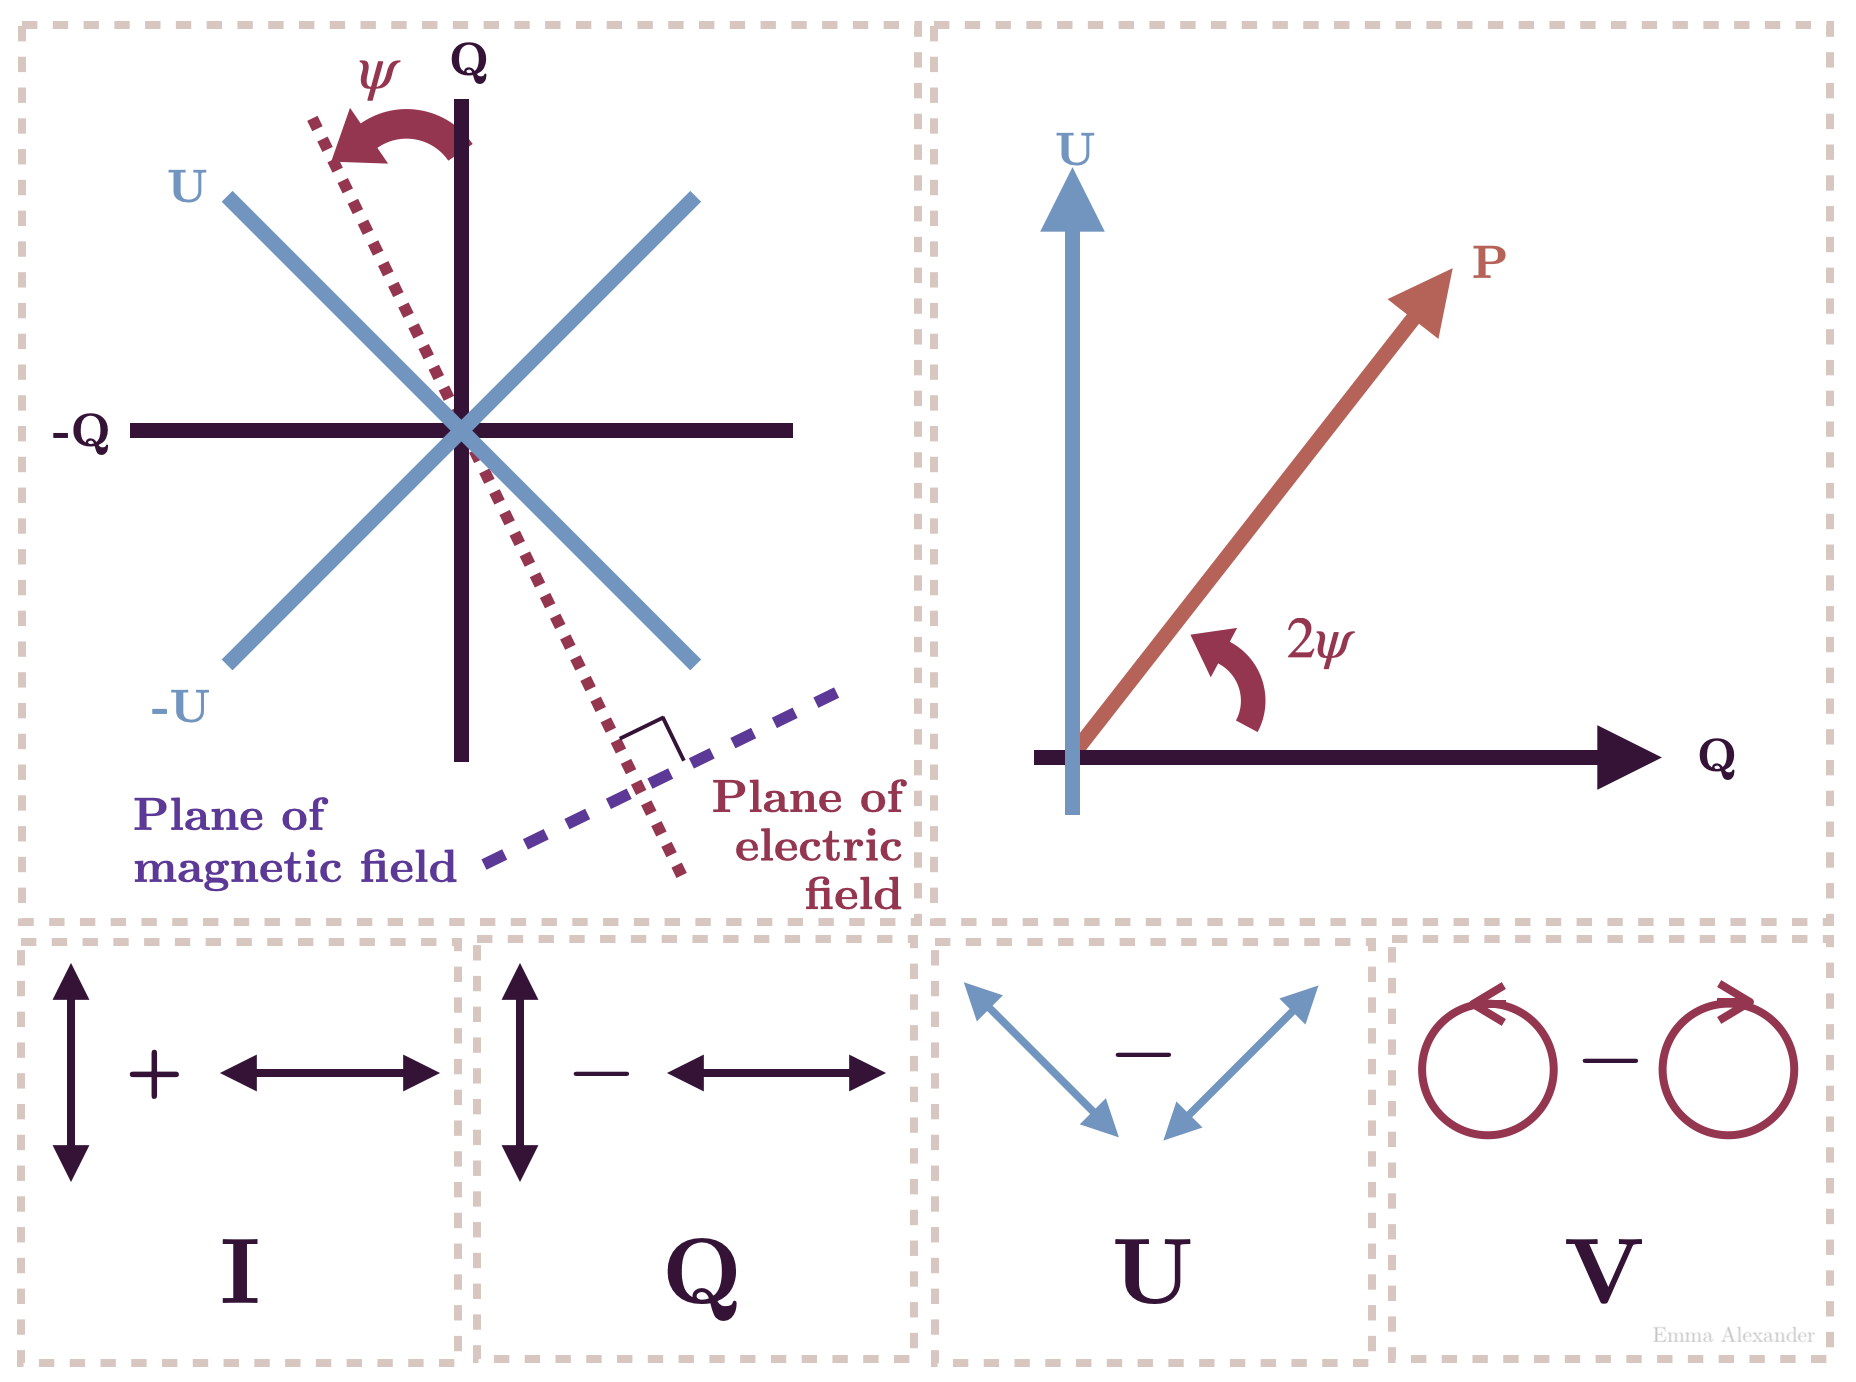
\includegraphics[width=0.5\linewidth]{figures/stokes.png}
    \caption{An illustration of the Stokes parameters. $I$ corresponds to total intensity (any direction of polarization), $Q$ gives the degree of preference for polarization along an axis, $U$ gives the degree of preference for polarization along the axis rotated $45^\circ$ from the first, and $V$ gives the degree of circular polarization.}
    \label{fig:stokes-parameters}
\end{figure}
